\documentclass[12pt]{article}
%%%%%%begin preamble
\usepackage[hmargin=1in, vmargin=1in]{geometry} % Margins
\usepackage{hyperref}
\usepackage{url}
\usepackage{natbib}
\usepackage{graphicx}
\usepackage{amsmath}
\usepackage{amsfonts}
\usepackage{amssymb}
\usepackage{wrapfig}

\usepackage{multicol}
\usepackage{etoolbox}
%\patchcmd{\thebibliography}{\section*{\refname}}
%    {\begin{multicols}{2}[\section*{\refname}]}{}{}
%\patchcmd{\endthebibliography}{\endlist}{\endlist\end{multicols}}{}{}


\usepackage[normalem]{ulem}
\usepackage{xcolor}
\newcommand{\edit}[2]{\textcolor{purple}{\sout{#1} \textbf{#2}}}

\hypersetup{
  colorlinks   = true,
  %citecolor    = blue
  citecolor    = blue
  % gray is not being found!?!
  % gray is found if pdfpages is used... crap.
  %citecolor    = grey
  %citecolor    = Gray
}


%% headers
\usepackage{fancyhdr}
\pagestyle{fancy}
\fancyhf{} % sets both header and footer to nothing
\lhead{Evan H. Anders}
\rhead{Exeter Draft Rutherford Proposal}
\cfoot{\footnotesize{\thepage}}
%\pagestyle{empty}
%\pagenumbering{gobble}
%\renewcommand*{\thefootnote}{\fnsymbol{footnote}}

\renewcommand{\vec}{\ensuremath{\boldsymbol}}
\newcommand{\dedalus}{\href{http://dedalus-project.org}{Dedalus}}
\newcommand{\del}{\ensuremath{\vec{\nabla}}}
\newcommand{\scrS}{\ensuremath{\mathcal{S}}}

\newcommand{\prf}{Physical Review Fluids}
\newcommand{\ssr}{Space Science Reviews}
\newcommand{\araa}{Annual Reviews of Astronomy and Astrophysics}
\newcommand{\mnras}{Monthly Notices of the Royal Astronomical Society}
\newcommand{\aap}{Astronomy \& Astrophysics}
\newcommand{\apjs}{The Astrophysical Journal Supplementary Series}
\newcommand{\apjl}{The Astrophysical Journal Letters}
\newcommand{\apj}{The Astrophysical Journal}

%\newcommand{\nosection}[1]{%
%  \refstepcounter{section}%
%  \addcontentsline{toc}{section}{\protect\numberline{\thesection}#1}%
%  \markright{#1}}
%\newcommand{\nosubsection}[1]{%
%  \refstepcounter{subsection}%
%  \addcontentsline{toc}{subsection}{\protect\numberline{\thesubsection}#1}%
%  \markright{#1}}

%\usepackage{atbegshi}
%%%%%%end preamble


%Make bibliography 2col
\bibliographystyle{apj_small}
\makeatletter
\renewenvironment{thebibliography}[1]
     {\begin{multicols}{2}[\paragraph*{\refname}\vspace{-0.1in}]%
      \@mkboth{\MakeUppercase\refname}{\MakeUppercase\refname}%
      \list{\@biblabel{\@arabic\c@enumiv}}%
           {\settowidth\labelwidth{\@biblabel{#1}}%
            \leftmargin\labelwidth
            \advance\leftmargin\labelsep
            \@openbib@code
            \usecounter{enumiv}%
            \let\p@enumiv\@empty
            \renewcommand\theenumiv{\@arabic\c@enumiv}}%
      \setlength{\itemsep}{-2pt}
      \sloppy
      \clubpenalty4000
      \@clubpenalty \clubpenalty
      \widowpenalty4000%
      \sfcode`\.\@m}
     {\def\@noitemerr
       {\@latex@warning{Empty `thebibliography' environment}}%
      \endlist\end{multicols}}
\makeatother



\begin{document}
\thispagestyle{fancy}
Convection is a crucial process in stellar astrophysics: it transports heat, generates magnetic fields, mixes chemical elements, and builds mean flows.
Despite this, many uncertainties remain regarding how to include convection in stellar models \citep{kaiser_etal_2020}, and these uncertainties profoundly impact other astrophysical disciplines, for example in causing uncertainty in the predicted masses of stellar remnants like black holes \citep{farmer_etal_2019}.
Space telescopes like NASA's \emph{Kepler} and \emph{TESS} missions and soon ESA's \emph{PLATO} mission provide datasets of $\gtrsim 10^{5-6}$ stars, but our ability to use the data from these telescopes is only as good as our models of the observed stars.
In the next five years, \textbf{I will work collaboratively with experts at Exeter to improve key uncertainties in stellar convection models and to build community tools which will help resolve future mysteries.}




\paragraph*{Task 1: Convective boundary mixing}
\begin{wrapfigure}{r}{0.3\textwidth}
	\begin{center}
	\vspace{-25pt}
    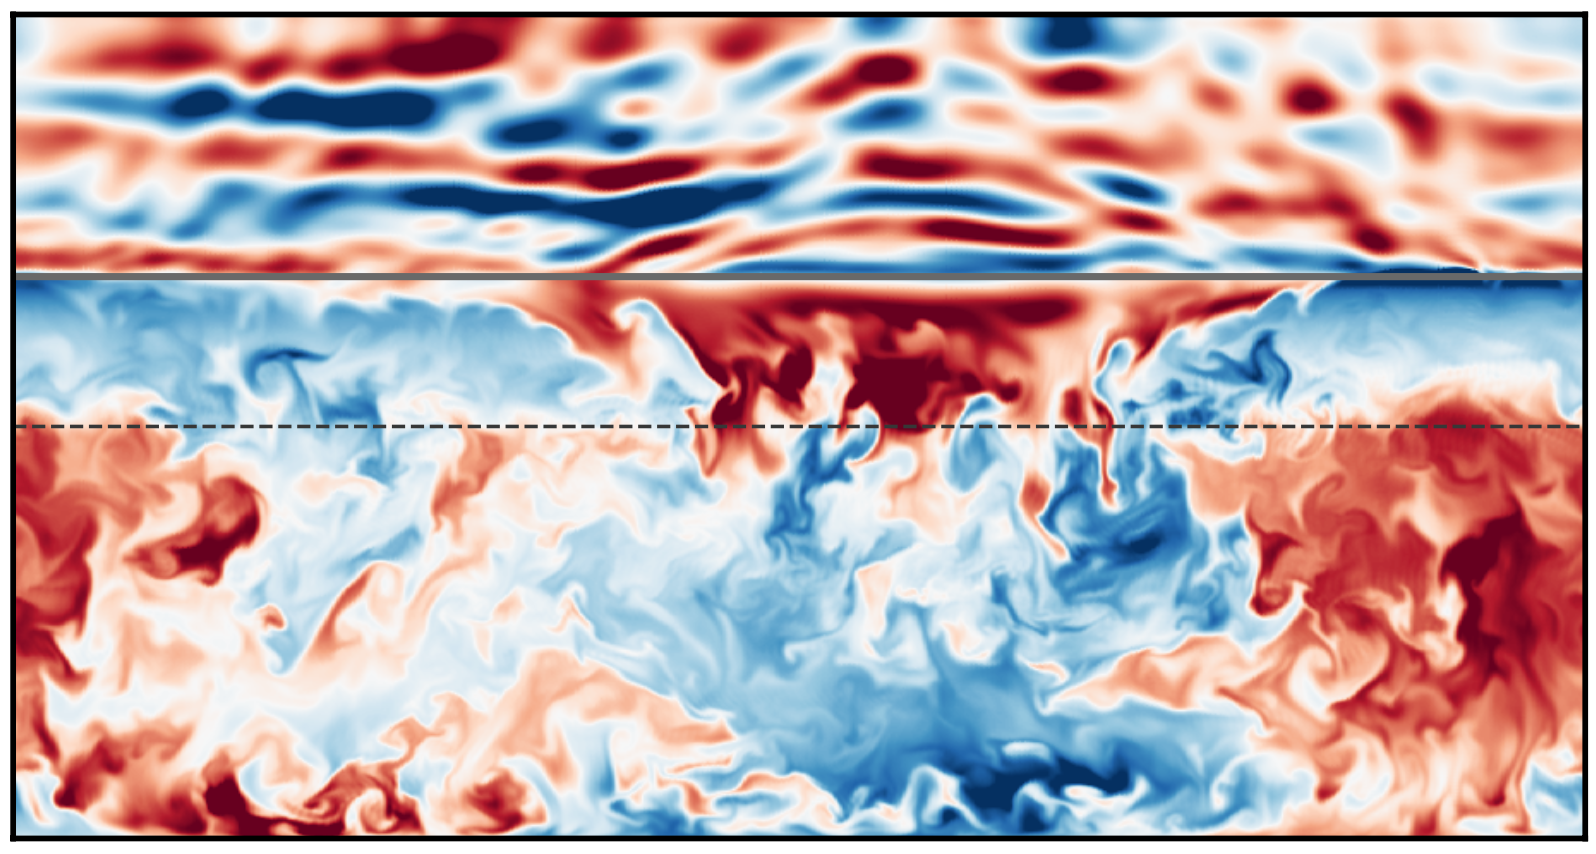
\includegraphics[width=0.28\textwidth]{./figs/penconv.png}
	\vspace{-16pt}
	\end{center}
    \caption{ A vertical slice of the temperature anomaly in a 3D simulation of penetrative convection.
	\label{fig:penconv} }
\end{wrapfigure}
The mixing at convective interfaces, broadly referred to as ``convective boundary mixing,'' is a compelling problem in modern theoretical astrophysics.
Inaccuracies in convective boundary mixing models lead to $\sim 50$\% uncertainties in the core masses of evolved, high-mass stars and substantial uncertainties in the lifetime of the star ($\sim$20\% on the main sequence, $\sim 5000$\% in the blue super-giant phase) \citep{kaiser_etal_2020}.
Observations of massive stars demonstrate unexpectedly high mixing at the core convection boundary \citep{johnston_2021}, and that convective boundary mixing must be ``fine-tuned'' as a function of stellar mass to match observations of stars in eclipsing binaries \citep{claret_torres_2018}.
Furthermore, asteroseismic observations \citep{pedersen_etal_2021} prefer a ``penetrative convection'' model: that is, one in which convective boundary mixing occurs efficiently in an extended region at the boundary of a convection zone.

In \citet{anders_etal_2022a}, I developed a theoretical model of penetrative convection, demonstrated its efficacy using 3D simulations such as the one in Fig.~\ref{fig:penconv}, and parameterized the theory for incorporation into 1D stellar evolution calculations.
We applied this parameterization using 1D stellar evolution calculations in \citet{jermyn_etal_2022}, and showed that our theory naturally reproduces the mass trend seen in eclipsing binary studies.
A great deal of work remains to be done in generalizing our theory of penetrative convection so that it works robustly in stellar interiors.
For example, the effects of rotation, composition gradients, magnetic fields, density stratification, and geometry (spherical vs.~Cartesian) have not yet been studied in detail.
%Furthermore, use of the fully compressible equations subtly changes the theoretical constraint that I derived, and must be explored.
In the coming years, I will expand this theory to include these effects while ensuring that this theory is incorporated self-consistently into the 1D stellar structure code MESA \citep{paxton_etal_2011}.
Exeter is the ideal place to carry out these studies in collaboration with Prof.~Baraffe and the ERC COBOM project team.
%My approach, which focuses on long-term thermal evolution of a penetrative zone will mesh complementarily with their focus on rare event statistics, and together we can make real progress towards solving this long-standing problem in stellar astrophysics.

\paragraph*{Task 2: Open-source, easily accessible code for global stellar simulations}
Large-scale, three-dimensional ``global'' models of stars allow us to investigate the observational manifestations of convective dynamics.
For example, recent observations have claimed the detection of waves driven by massive star core convection \citep{bowman_etal_2019}.
These observations should be directly compared to the surface manifestation of convectively-driven waves in 
%Such a wave signal could resolve disagreements about convective excitation mechanisms and the transfer of waves through stellar interiors \citep{rogers_etal_2013,lecoanet_etal_2021}.
\begin{wrapfigure}{l}{0.3\textwidth}
	\begin{center}
	\vspace{-30pt}
    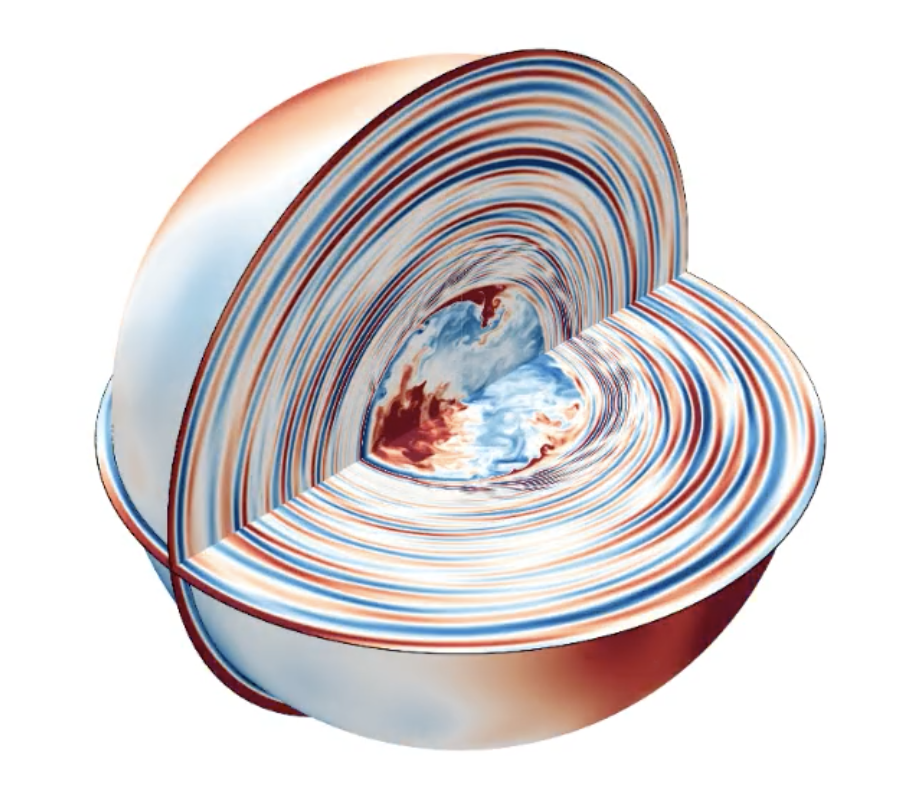
\includegraphics[width=0.28\textwidth]{./figs/massive_star.png}
	\vspace{-20pt}
	\end{center}
    \caption{ A volume rendering of scaled entropy fluctuations in a Dedalus simulation of a 40 $M_\odot$ star.
	\label{fig:massive_star} }
	\vspace{-10pt}
\end{wrapfigure}
simulations such as the one I created which is pictured in Fig.~\ref{fig:massive_star}.
Unfortunately, there are no open-source, user-friendly codes for running dynamical simulations of stars.
Current stellar dynamics codes require help from an expert to run, are restricted to limited equation sets, or only focus on a portion of the stellar domain.
Over the next five years, I will build an easy-to-use Python module that uses the Dedalus pseudospectral framework \citep{burns_etal_2020} so that the broader community has access to the tools to run simulations like the one in Fig.~\ref{fig:massive_star}.
The background stellar stratification is realistic and is imported from MESA stellar models \citep{paxton_etal_2011}.
Planned evolutionary equation sets will include both hydrodynamic and magnetohydrodynamic formulations. %of both the anelastic and fully compressible equations.
I have eight years of experience using Dedalus to study convective dynamics and a track record of publishing open-source, open-access scientific code.
Exeter is the ideal place to develop this module thanks to local expertise such as Prof.~Browning's knowledge of dynamo simulations of massive stars and Prof.~Baraffe's experience developing the MUSIC code and working on lower-mass stars.


\paragraph*{Task 3: Convection at the smallest scales}
\begin{wrapfigure}{r}{0.25\textwidth}
	\begin{center}
	\vspace{-30pt}
    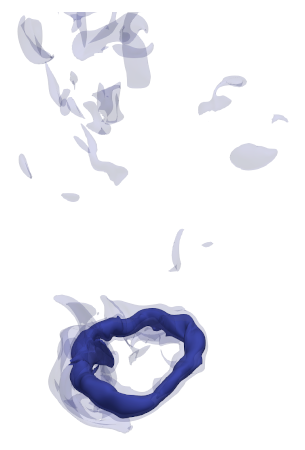
\includegraphics[width=0.23\textwidth]{./figs/turbulent_thermal.png}
	\vspace{-16pt}
	\end{center}
    \caption{ A volume rendering of an evolved thermal in its buoyant vortex ring state.
    Packets of buoyant fluid lost during its spin-up can be seen above it in its wake.
	\label{fig:thermal} }
\end{wrapfigure}
There is a ``convective conundrum'' in observations of the Sun:``giant cells'' predicted by theory and simulations are not detected by many observations \citep{hanasoge&all2012,proxauf_2021}.
One proposed hypothesis to this conundrum is the ``entropy rain hypothesis,'' which posits that a large portion of the solar flux may be carried by small, cold downflows.
These downflows may be so efficient at carrying heat that giant cells may not be necessary for the Sun to remain in thermal equilibrium.
In \citet{andersLB2019} I studied the evolution of single convective downflows which I modeled as ``thermals,'' or cold fluid blobs which fall buoyantly and evolve into vortex rings (as in Fig.~\ref{fig:thermal}).
We surprisingly found that these small-scale features could easily carry the solar luminosity, but there are still many areas of uncertainty that I will study in the next 5 years.
The effects of turbulent entrainment and rotation on these cold ``raindrops'' is unclear; these processes may dilute or deflect the raindrops, decreasing their ability to transport heat.
Furthermore, many argue that the thermal model (a finite cold fluid parcel) is a poor model for solar downflows, preferring a plume model (which has a continuous cold source).
I will build upon modern plume models \citep[e.g.,][]{tarshish_romps_2022} to account for the effects of density stratification and rotation in the Sun to determine if the plume-generated entropy rain can carry the solar luminosity.
Thermals and plumes are frequently investigated in the geophysical context, and I look forward to collaborating with experts on geophysical fluid dynamics at Exeter such as Prof.~Vallis as I carry out these studies.


%{\scriptsize
{\small
\bibliography{biblio}
}
\end{document}
